% !TeX program = pdflatex
% =============================================================================
% Aufgabenblatt: Kondensatoren
% UZH Praktikum I -- Sara Romer Urban, Kantonsschule im Lee, HS2026
% Klassen: 4fh (regulaer, 25.08.2026) + 4cdeg (SP4, 28.08.2026) -- gemeinsames
% Material (siehe institutionen/UZH-Praktikum-I/CLAUDE.md, Abschnitt "SP
% (Schwerpunktfach) vs. regulaere Physik").
%
% Enthaelt ausschliesslich die PhET-/Excel-Lernaufgabe (Kapazitaet mit der
% Simulation "Capacitor Lab: Basics" bestimmen, Teil 1-4), die die SuS zu
% zweit am Computer bearbeiten -- Aufgaben, die eine Simulation oder Excel
% brauchen, gehoeren ins Aufgabenblatt, unabhaengig vom Zeitpunkt der
% Bearbeitung. Sortieraufgabe, die Herleitungs-Uebung zum Dielektrikum,
% Theorie und alles im Plenum Behandelte stehen in
% arbeitsblatt4-kondensatoren-teil1.tex; reine Vor-/Nachbereitungs-Uebungen
% in kondensatoren-zusatzaufgaben.tex.
%
% Quellen: lernziele.md (dieser Ordner), kondensatoren-notizen-sara-romer.txt
% (Besprechungsnotizen von Sara Romer), Vorwissen/Elektrostatik/ (Coulombkraft,
% E-Feld, Potential/Spannung -- bereits bekannt, hier nur repetiert), sowie die
% Referenzquellen direkt in diesem Ordner (LEIFIphysik, Physik Libre 12.11,
% HSHL "Lerninhalte und Abschlussarbeiten" -- von Letzterem nur die
% Wassereimer-Analogie und die qualitative Beschreibung, nicht die dortige
% Integral-/Ableitungsrechnung, die Hochschulstoff ist).
% =============================================================================
\documentclass[addpoints,11pt,a4paper]{exam}

\usepackage[T1]{fontenc}
\usepackage[utf8]{inputenc}
\usepackage[ngerman]{babel}
\usepackage{lmodern}
\usepackage[a4paper,margin=2.2cm,headheight=14pt]{geometry}
\usepackage{amsmath}
\usepackage{siunitx}
% Hausstil: zusammengesetzte Einheiten immer als echter Bruch (\frac), nicht
% als Inline-Schrägstrich oder \tfrac -- gilt global für jedes \si/\SI.
\sisetup{per-mode=fraction,fraction-command=\frac}
\usepackage{array,booktabs,tabularx,multirow}
\usepackage{enumitem}
\usepackage{xcolor}
\usepackage{colortbl}
\usepackage{tikz}
\usepackage{physics}
\usepackage{circuitikz}
\usepackage[most]{tcolorbox}
\usepackage{lastpage}
\usepackage{graphicx}
\usepackage{hyperref}

\usetikzlibrary{arrows.meta,calc,angles,quotes}

\usepackage{setspace}
\usepackage{needspace}
\setlength{\parindent}{0pt}
\setlength{\parskip}{0.6em}
\setstretch{1.08}
\setlist[itemize]{itemsep=0.4em}

% -----------------------------
% Farben (Corporate-Farbschema Physik KFR)
% -----------------------------
\definecolor{titleblue}{HTML}{183A6B}
\definecolor{accentblue}{HTML}{2E6F9E}
\definecolor{lightblue}{HTML}{EAF4FB}
\definecolor{verylightblue}{HTML}{F7FBFE}
\definecolor{lightgray}{HTML}{F4F6F8}
\definecolor{darkgray}{HTML}{4A4A4A}
\definecolor{accentorange}{HTML}{D9720C}
\definecolor{accentpurple}{HTML}{7B2D8E}
% Theorie-Block: eigene Farbe (grün).
\definecolor{theorygreen}{HTML}{2E7D4F}
\definecolor{lighttheorygreen}{HTML}{EAF7EF}
% Gruppenarbeit-Box: eigene Farbe (Petrol/Teal).
\definecolor{groupteal}{HTML}{1B7F72}
\definecolor{lightgroupteal}{HTML}{E8F5F3}
% Hinweisbox: Orange (accentorange), für wichtige Klarstellungen.
\definecolor{lightorange}{HTML}{FCEEE0}
% Formelbox: Violett (accentpurple), für die zentralen Formeln dieser Einheit.
\definecolor{lightpurple}{HTML}{F3EAF7}

% Links (hyperref): farblich ans Corporate-Farbschema angeglichen.
\hypersetup{
  colorlinks=true,
  urlcolor=accentblue,
  linkcolor=accentblue,
  pdftitle={Aufgabenblatt 3: Kondensatoren},
  pdfauthor={Loris Keller}
}

% -----------------------------
% Spaltentypen
% -----------------------------
\newcolumntype{Y}{>{\centering\arraybackslash}X}
\newcolumntype{P}[1]{>{\raggedright\arraybackslash}p{#1}}

% -----------------------------
% Boxen
% -----------------------------
\tcbset{before skip=10pt, after skip=10pt}
\newtcolorbox{titlebox}{
  enhanced,
  colback=titleblue,
  colframe=titleblue,
  boxrule=0pt,
  arc=3mm,
  left=3mm,right=3mm,top=3mm,bottom=3mm
}

\newlength{\aufgabenindent}
\settowidth{\aufgabenindent}{10.\hskip\labelsep}

% Praktikum I: Lernziele/Einleitung/Theorie/Aufgaben werden NICHT mehr
% farbig gerahmt (nur Formel-, Hinweis- und Antwortbox bleiben Boxen) --
% siehe institutionen/UZH-Praktikum-I/CLAUDE.md, Abschnitt "Boxen-Layout".
\newenvironment{infobox}{%
  \par\addvspace{10pt}\noindent
}{%
  \par\addvspace{10pt}
}

\newenvironment{theoriebox}[1][Theorie]{%
  \par\addvspace{10pt}\noindent\textbf{#1}\par\smallskip\noindent
}{%
  \par\addvspace{10pt}
}

% taskbox/groupbox stehen in questions VOR dem ersten \question (Bilder,
% Fliesstext) -- exam.cls' questions-Liste braucht dafür eine echte,
% eigenständige Box (sonst "Something's wrong--perhaps a missing \item",
% weil z.B. ein \begin{center} vor dem ersten \item der Aussenliste steht).
% Deshalb bleiben es tcolorboxen, nur unsichtbar gemacht (keine Farbe/Rahmen,
% kein Padding) statt sie durch reine Absätze zu ersetzen.
\newtcolorbox{taskbox}[1][]{
  enhanced, breakable,
  colback=white, colframe=white, boxrule=0pt,
  left=0mm,right=0mm,top=0mm,bottom=0mm,
  before skip=10pt, after skip=10pt,
  before upper={%
    \def\tmpboxtitle{#1}%
    \ifx\tmpboxtitle\empty\else\noindent\textbf{#1}\par\smallskip\fi
  }
}

\newtcolorbox{groupbox}[1][Gruppenarbeit]{
  enhanced, breakable,
  colback=white, colframe=white, boxrule=0pt,
  left=0mm,right=0mm,top=0mm,bottom=0mm,
  before skip=10pt, after skip=10pt,
  before upper={\noindent\textbf{#1}\par\smallskip}
}

% beispielbox: für die Einleitung und für durchgerechnete Beispiele
% innerhalb der Theorie -- wie die anderen Inhaltsboxen ungerahmt.
\newenvironment{beispielbox}[1][Beispiel]{%
  \par\addvspace{10pt}\noindent\textbf{#1}\par\smallskip\noindent
}{%
  \par\addvspace{10pt}
}

% hinweisbox: Orange, für wichtige Klarstellungen/Verwechslungswarnungen.
\newtcolorbox{hinweisbox}[1][Hinweis]{
  enhanced,
  breakable,
  colback=lightorange,
  colframe=accentorange,
  title={#1},
  fonttitle=\bfseries,
  boxrule=0.7pt,
  arc=2mm,
  left=5mm,right=5mm,top=2mm,bottom=2mm
}

% formelbox: Violett, um die zentralen Formeln dieser Einheit hervorzuheben.
\newtcolorbox{formelbox}[1][Formel]{
  enhanced,
  breakable,
  colback=lightpurple,
  colframe=accentpurple,
  title={#1},
  fonttitle=\bfseries,
  boxrule=0.9pt,
  arc=2mm,
  left=5mm,right=5mm,top=2mm,bottom=2mm
}

\newtcolorbox{answerbox}{
  breakable,
  colback=white,
  colframe=gray!55,
  boxrule=0.5pt,
  arc=1.5mm,
  left=2mm,right=2mm,top=2mm,bottom=2mm
}

% teilkopf: fette Zwischenüberschrift zur klaren Abgrenzung der Teile 1-4
% innerhalb der langen Lernaufgabe -- ungerahmt, wie die anderen
% Inhaltsboxen.
\newenvironment{teilkopf}{%
  \par\addvspace{8pt}\noindent\bfseries\sffamily
}{%
  \par\addvspace{6pt}
}

% Marke: kleines farbiges Inline-Label für Teilschritte (z.B. "Schritt 1")
% und Ergebnis-Callouts innerhalb einer Aufgabe. Standardfarbe Violett (wie
% formelbox); über das optionale Argument umschaltbar, z.B. \Marke[accentorange]{...}.
\newtcbox{\Marke}[1][accentpurple]{
  nobeforeafter,
  colback=#1,
  colframe=#1,
  coltext=white,
  boxrule=0pt,
  arc=2pt,
  left=5pt,right=5pt,top=2pt,bottom=2pt,
  fontupper=\bfseries\sffamily\small
}

% --- Lösungen ein-/ausblenden -----------------------------------------------
%\noprintanswers
\printanswers

\pointformat{}
\renewcommand{\solutiontitle}{\noindent\color{titleblue}\textbf{Lösung:}\enspace}

\pagestyle{headandfoot}
\cfoot{\textcolor{darkgray}{Seite \thepage\ von \pageref{LastPage}}}

\newcommand{\Kopfzeile}[4]{%
  \begin{titlebox}
    {\color{white}\sffamily\bfseries\Large #4}
  \end{titlebox}
  \vspace{0.5em}
  \noindent\textbf{Klasse:}~#1 \hfill \textbf{Datum:}~#2 \hfill \textbf{Thema:}~#3
    \hfill \textbf{Lehrperson:}~Loris Keller
  \vspace{0.8em}
  \lhead{\textcolor{darkgray}{#3}}
  \rhead{\textcolor{darkgray}{#4}}
}

\newlength{\antwortraumlen}
\newcommand{\Antwortraum}[1]{%
  \pgfmathsetlength{\antwortraumlen}{#1*2.5cm}%
  \begin{answerbox}
    \rule{0pt}{\antwortraumlen}%
  \end{answerbox}%
}

% Werte für Kopfzeile zentral setzen
\newcommand{\Klasse}{4fh / 4cdeg (SP4)}
\newcommand{\Datum}{25.08.2026 (4fh) / 28.08.2026 (4cdeg)}
\newcommand{\Thema}{Kondensatoren}
\newcommand{\ArbeitsblattTitel}{Aufgabenblatt 3: Kondensatoren}

\begin{document}

\Kopfzeile{\Klasse}{\Datum}{\Thema}{\ArbeitsblattTitel}

% =============================================================================
% Lernaufgabe
% =============================================================================
\begin{questions}
\begin{groupbox}[Lernaufgabe (Partnerarbeit): Kapazität mit der PhET-Simulation bestimmen]
\noindent
\begin{minipage}[c]{1.8cm}
  \href{https://phet.colorado.edu/de/simulations/capacitor-lab-basics}{%
    
\includegraphics[width=1.6cm]{Bilder/phet-logo-trademarked.png}}
\end{minipage}%
\begin{minipage}[c]{\dimexpr\linewidth-1.8cm\relax}
Öffnen Sie zu zweit die Simulation
\href{https://phet.colorado.edu/de/simulations/capacitor-lab-basics}{\glqq Capacitor Lab: Basics\grqq{}}.
\end{minipage}

\begin{center}
  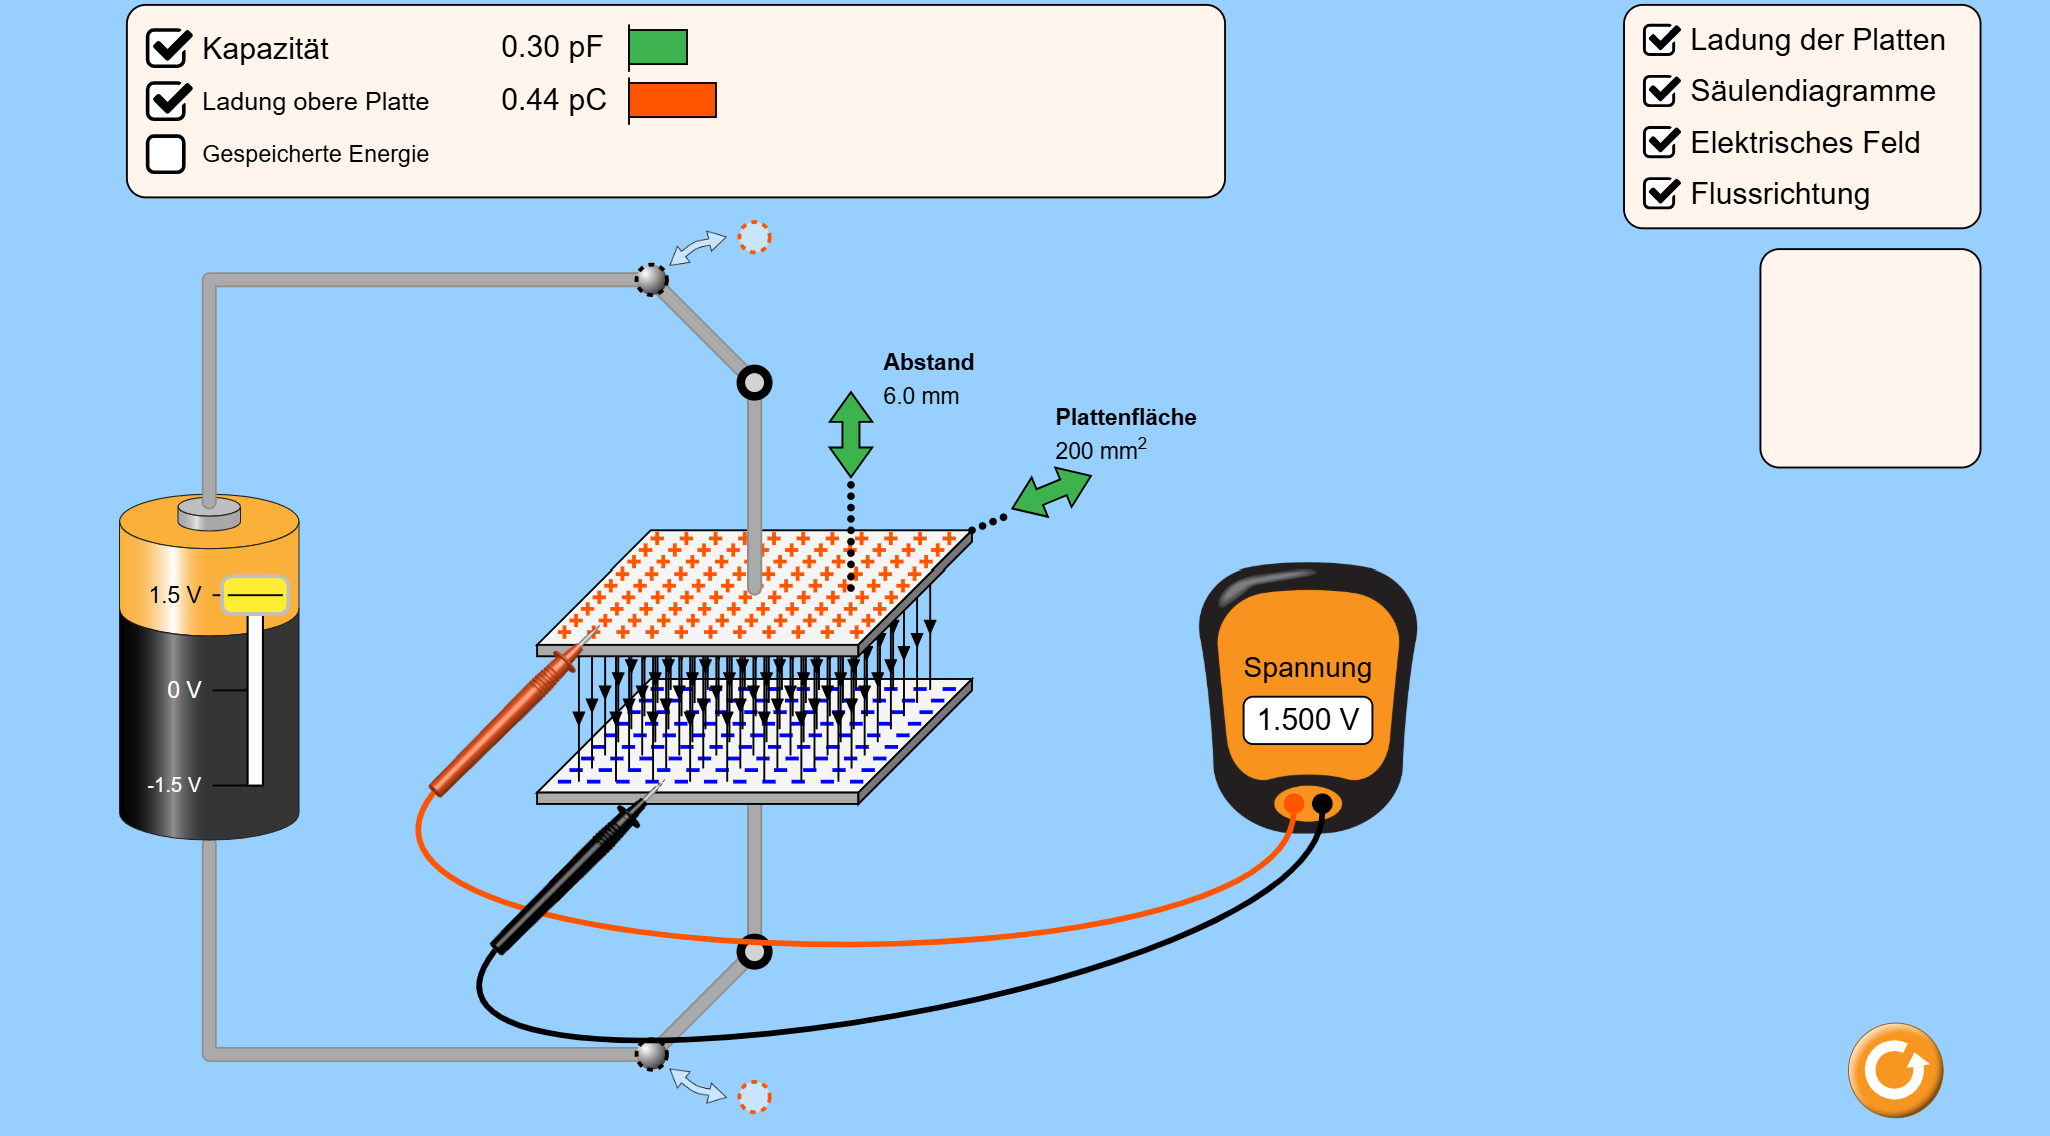
\includegraphics[width=10cm]{Bilder/Phet_Kapazitaet.png}
\end{center}
{\scriptsize So sieht der Einstiegsscreen der Simulation aus: Links die
Anzeigen für Kapazität und Ladung, in der Mitte der Plattenkondensator mit
verstellbarer Plattenfläche und verstellbarem Abstand, rechts das
Multimeter für die Spannung.}

\noindent
\begin{minipage}[c]{1.8cm}
  
\includegraphics[width=1.6cm]{Bilder/excel_logo.jpg}
\end{minipage}%
\begin{minipage}[c]{\dimexpr\linewidth-1.8cm\relax}
Laden Sie ausserdem die Excel-Datei \texttt{kondensatoren-phet-messvorlage.xlsx}
herunter und tragen Sie darin Ihre Messwerte ein.
\end{minipage}

\begin{hinweisbox}[Die vier Excel-Blätter]
\begin{itemize}[leftmargin=1.2cm,itemsep=0.2em]
  \item \texttt{Anleitung}: kurze Übersicht über alle vier Teile.
  \item \texttt{Teil 1 - U und Q}: für Teil 1.
  \item \texttt{Teil 2a - A und C}: für Teil 2, Fläche $A$ variieren.
  \item \texttt{Teil 2b - d und C}: für Teil 2, Abstand $d$ variieren.
\end{itemize}
Nur die weissen Zellen ausfüllen: Diagramme und Trendlinien
aktualisieren sich automatisch.
\end{hinweisbox}

\question

\begin{teilkopf}
Teil 1: Zusammenhang zwischen $Q$, $U$ und $C$
\end{teilkopf}
Die Lehrperson zeigt dieses erste Blatt zunächst gemeinsam am Beamer
(Simulation und Excel-Blatt \texttt{Teil 1 - U und Q}). Der Kondensator
bleibt während der ganzen Messreihe an der Batterie angeschlossen.
Übertragen Sie danach dieselben Schritte auf Ihre eigenen Messwerte:
\needspace{5cm}
\begin{enumerate}[leftmargin=1.4cm,itemsep=0.2em]
  \item Halten Sie die Geometrie (Fläche $A$, Abstand $d$) konstant.
  \item Verändern Sie die Spannung $U$ in mindestens 5 Schritten und lesen
  Sie jeweils -- bei angeschlossener Batterie und konstant gehaltenem $U$
  -- die Ladung $Q$ ab (Voltmeter einschalten, Messspitzen an die obere
  und die untere Platte halten).
  \item Tragen Sie $U$ und $Q$ ins Excel-Blatt \texttt{Teil 1 - U und Q}
  ein: Diagramm und Trendlinie erscheinen automatisch.
\end{enumerate}
\begin{parts}
  \needspace{10cm}
  \part[3] Beschreiben Sie mit Ihrem Diagramm den Zusammenhang zwischen
  $Q$ und $U$: Welchen Funktionstyp erkennen Sie, und was könnte die
  Steigung der Trendlinie physikalisch bedeuten? Sie vergleichen Ihr
  Resultat gleich im Plenum mit einem zweiten Kondensator.
  \Antwortraum{3}
  \begin{solution}
  \begin{center}
    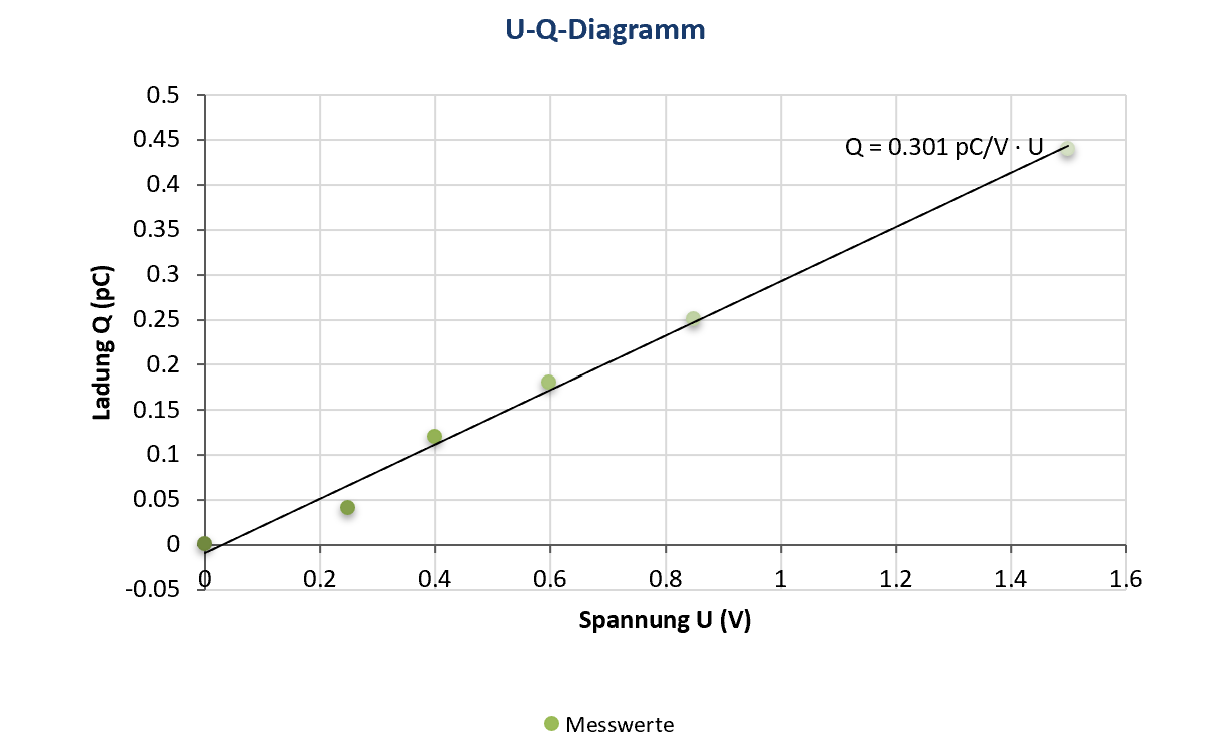
\includegraphics[width=8cm]{Bilder/Loesung_Teil1.png}
  \end{center}
  Einen linearen, proportionalen Zusammenhang ($Q\sim U$): Die Messpunkte
  liegen auf einer Ursprungsgeraden. Die Steigung der Trendlinie
  entspricht der Kapazität $C$ des eingestellten Kondensators.
  \end{solution}

  \part[2] Vergleichen Sie die abgelesene Kapazität mit dem Wert, den die
  Simulation direkt anzeigt. Stimmen die Werte überein?
  \Antwortraum{2}
  \begin{solution}
  Ja, die aus der Steigung der Trendlinie abgelesene Kapazität sollte (im
  Rahmen der Ablesegenauigkeit) mit dem von der Simulation angezeigten Wert
  übereinstimmen.
  \end{solution}
\end{parts}

\question

\begin{teilkopf}
Teil 2: Einfluss von Fläche und Abstand
\end{teilkopf}
Die nächste Simulationsansicht zeigt die Kapazität direkt an. Der
Kondensator bleibt dabei an der Batterie angeschlossen, die Spannung $U$
bleibt konstant. Untersuchen Sie, wie die Kapazität von der Geometrie
abhängt.
\begin{parts}
  \part[3] Öffnen Sie das Excel-Blatt \texttt{Teil 2a - A und C}. Halten
  Sie den Plattenabstand $d$ konstant und notieren Sie seinen Wert in der
  dafür vorgesehenen Zelle. Verändern Sie die Plattenfläche $A$, tragen
  Sie die Werte ein und beschreiben Sie den Zusammenhang im Diagramm.
  \Antwortraum{3}
  \begin{solution}
  \begin{center}
    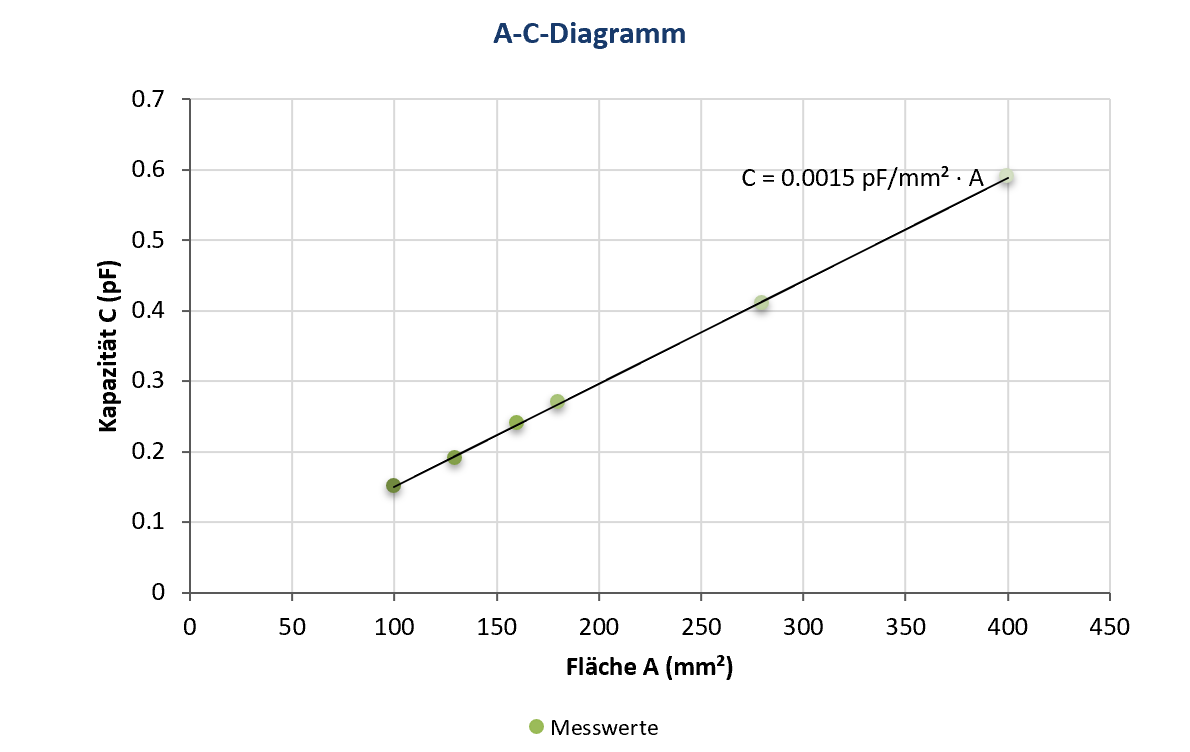
\includegraphics[width=8cm]{Bilder/Loesung_Teil2a.png}
  \end{center}
  $C$ wächst proportional zu $A$ (Ursprungsgerade im $A$-$C$-Diagramm, bei
  konstantem $d$): $C \sim A$.
  \end{solution}

  \part[3] Öffnen Sie das Excel-Blatt \texttt{Teil 2b - d und C}. Halten
  Sie nun die Plattenfläche $A$ konstant und notieren Sie ihren Wert in
  der dafür vorgesehenen Zelle. Verändern Sie den Plattenabstand $d$,
  tragen Sie die Werte ein und beschreiben Sie den Zusammenhang im
  Diagramm.
  \Antwortraum{3}
  \begin{solution}
  \begin{center}
    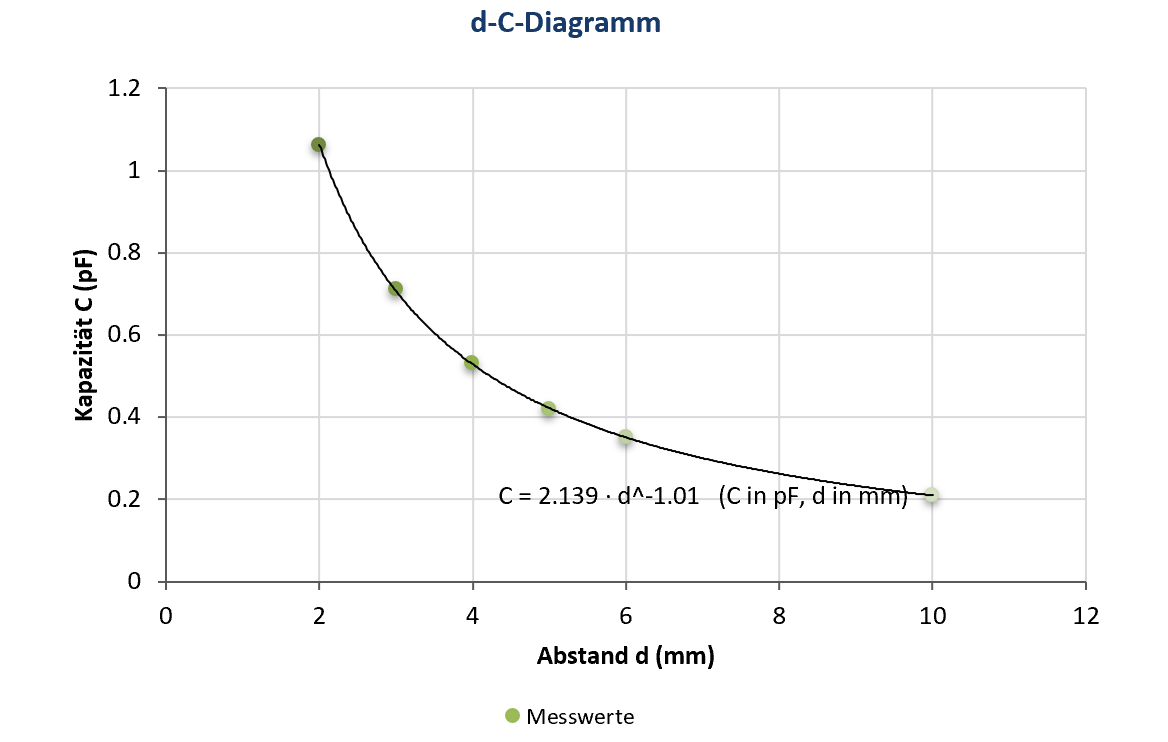
\includegraphics[width=8cm]{Bilder/Loesung_Teil2b.png}
  \end{center}
  $C$ nimmt mit wachsendem $d$ ab, und zwar umgekehrt proportional:
  $C \sim \frac{1}{d}$ (bei konstantem $A$).
  \end{solution}

  \Marke[accentorange]{Eure Kondensatorformel}, im Plenum hergeleitet
  (siehe Arbeitsblatt 4), bitte in eigener Handschrift eintragen:
  \Antwortraum{1}
  \begin{solution}
  \[
    C = \varepsilon_0\cdot\frac{A}{d}.
  \]
  \end{solution}
\end{parts}

\question

\begin{teilkopf}
Teil 3: Kondensator von der Batterie getrennt
\end{teilkopf}
Bleiben Sie auf demselben Screen wie in Teil 1/2. Laden Sie den Kondensator
wie in Teil 1 auf und trennen Sie ihn danach von der Batterie (Schalter in
der Simulation öffnen).
\begin{parts}
  \part[2] Verändern Sie nun den Plattenabstand $d$. Welche Grösse bleibt
  dabei konstant, welche ändert sich? Begründen Sie mit $Q=C\cdot U$.
  \Antwortraum{2}
  \begin{solution}
  Da der Kondensator von der Spannungsquelle getrennt ist, kann keine
  Ladung mehr zu- oder abfliessen: Die Ladung $Q$ bleibt konstant. Der
  Plattenabstand $d$ verändert dagegen die Kapazität
  $C=\varepsilon_0\cdot\frac{A}{d}$, also muss sich gemäss $Q=C\cdot U$
  die Spannung $U$ anpassen.
  \end{solution}

  \needspace{7cm}
  \part[2] Was passiert konkret mit der Spannung $U$, wenn Sie $d$
  vergrössern? Überprüfen Sie Ihre Vorhersage in der Simulation.
  \Antwortraum{2}
  \begin{solution}
  Wird $d$ vergrössert, so wird $C$ kleiner (da $C\sim\frac{1}{d}$). Weil
  $Q$ konstant bleibt, muss $U=\frac{Q}{C}$ steigen: Die Spannungsanzeige
  der Simulation nimmt zu.
  \end{solution}
\end{parts}

\question[3]

\begin{teilkopf}
Teil 4: Leuchtdauer im Simulationsscreen \glqq Light Bulb\grqq{}
\end{teilkopf}
Wechseln Sie zum zweiten Screen der Simulation, wo der Kondensator statt an
eine Batterie an eine Glühbirne angeschlossen ist.
\begin{center}
  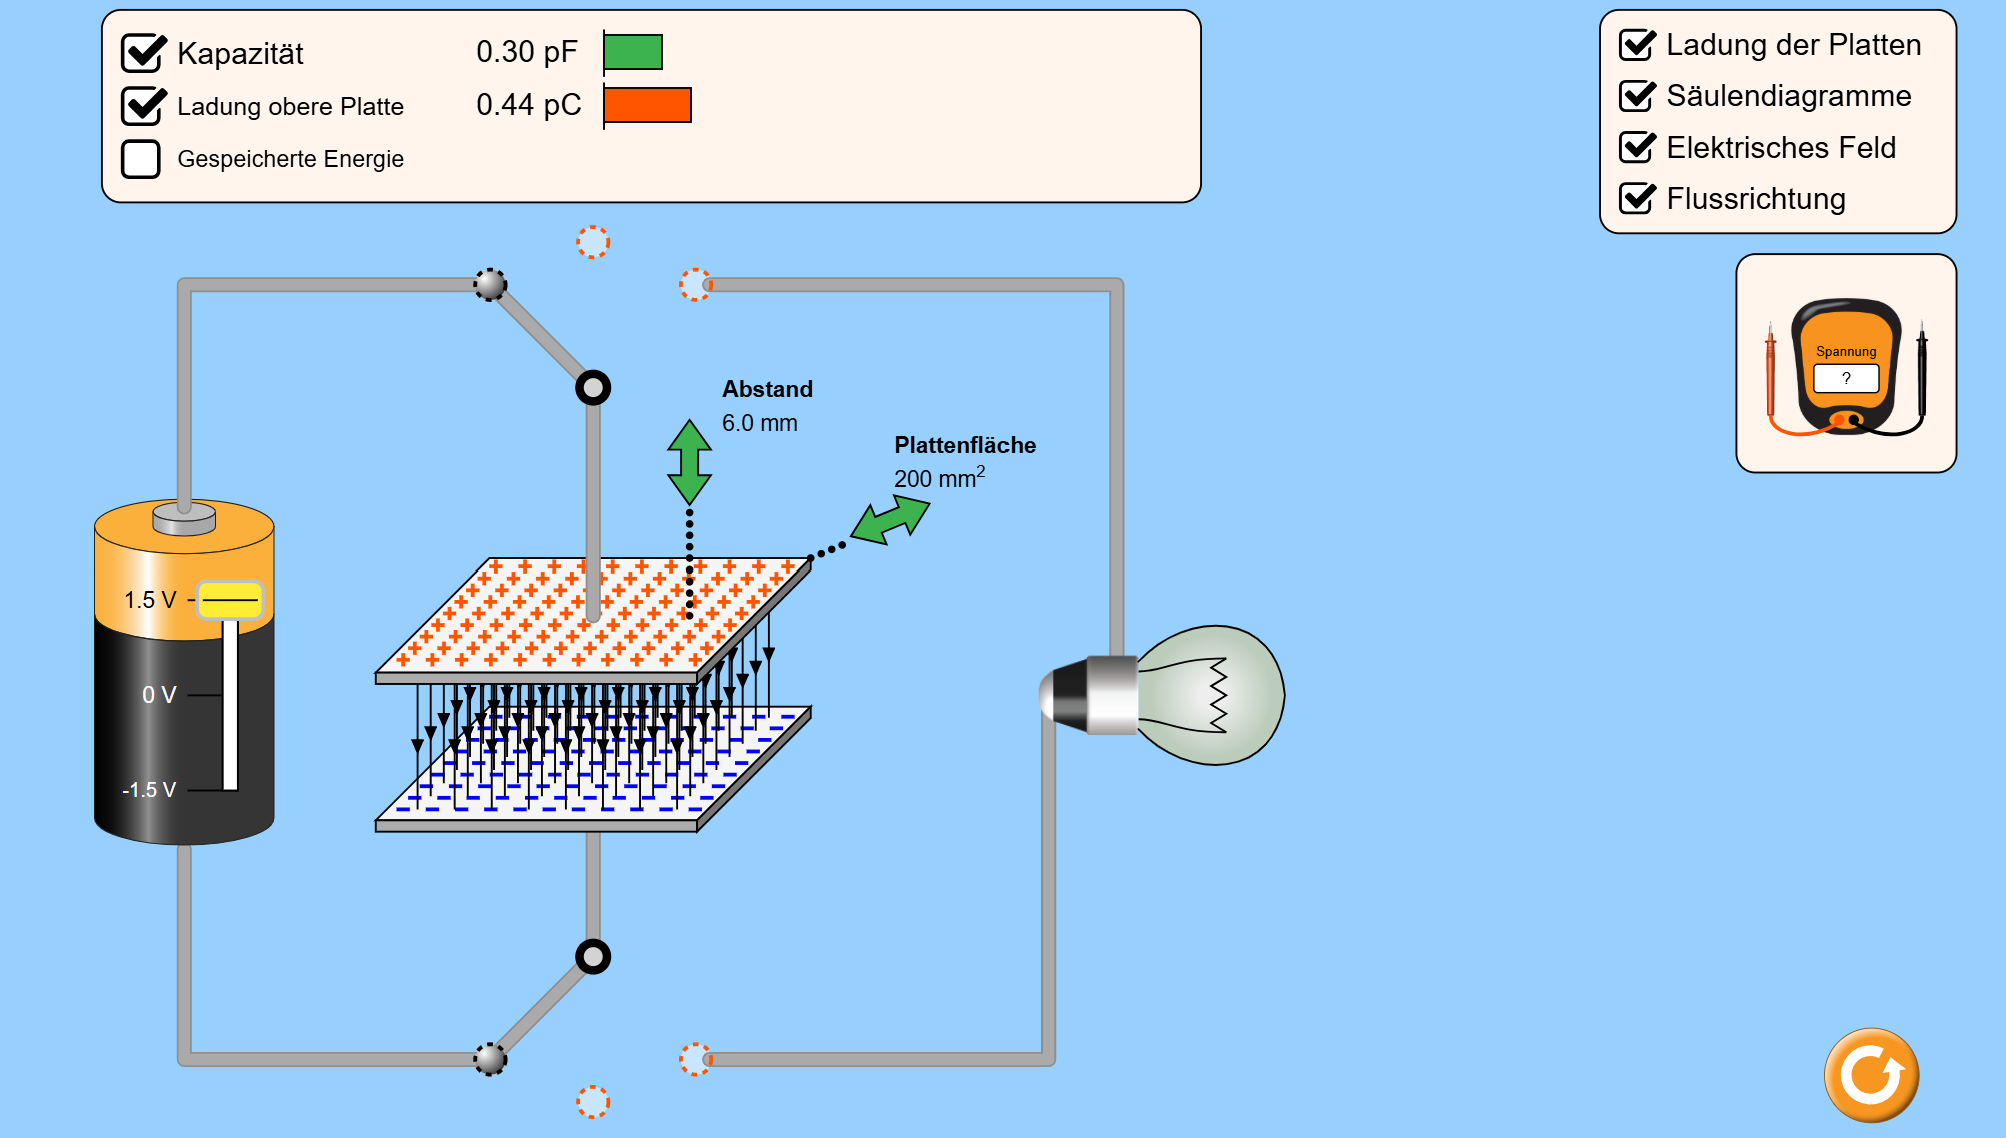
\includegraphics[width=9cm]{Bilder/Phet_Lichtquelle.png}
\end{center}
{\scriptsize Der Screen \glqq Light Bulb\grqq{}: Batterie, Kondensator und
Glühbirne im selben Stromkreis.}

Bestätigen Sie hier am Computer die Beobachtung aus dem
Entladeexperiment: Laden Sie zwei Kondensatoren mit unterschiedlicher
Kapazität (z.\,B. über die Plattenfläche $A$) bei angeschlossener Batterie
und derselben, konstant gehaltenen Spannung $U$ auf. Trennen Sie sie
danach von der Batterie und lassen Sie sie über die Glühbirne entladen.
Begründen Sie zusätzlich mit $Q=C\cdot U$, weshalb der Kondensator mit der
grösseren Kapazität mehr Ladung enthält.
\Antwortraum{3}
\begin{solution}
Wie im Demoversuch vorhergesagt, leuchtet die Glühbirne beim Kondensator
mit grösserer Kapazität länger. Da $U$ bei beiden Kondensatoren gleich
ist, folgt aus $Q=C\cdot U$ direkt: Ein grösseres $C$ bedeutet ein
grösseres $Q$, also mehr Ladung, die über die Glühbirne abfliessen muss.
\end{solution}
\end{groupbox}
\end{questions}

\end{document}
